\chapter{序論}
\label{chap_intro}

\section{研究背景}
胃がんは,日本でもっとも罹患数が多いがんであり,年間13万人が罹患し5万人が亡くなっている.内視鏡の生検は食道,大腸,小腸,胃などを鉗子で2 mm角程度の立方体で抜き出し,染色したものを2,3断面にカットしてから病理診断医が顕微鏡で観察,診断している.断面のみの観察では内部に腫瘍がある場合に見落としてしまうリスクがあるため,本研究では組織透明化技術を用いて検体を丸ごと観察することを試みた.

病理医が全てを診断するには負担が大きいこと,病変の見落としリスクがあること,経験を詰んだ医師でも判断の難しい病変を見つけることが求められている.

内視鏡で見つけた病変が,腫瘍か非腫瘍かを判別したり,その悪性度を判定したりすることは生検を観察する必要がある.内視鏡検査の専門医のマンパワーが不足している.現在の日本の病理の専門医は2483名\cite{pathology}で,その人数に対して標本500万件を年間で処理している現状である.

また癌検診では,担当医が判定して専門医がダブルチェックをしているが,AIがスクリーニングを行って専門医の確認が必要な症例を絞り込む.専門医の判定は主観的であることや,専門医ごとにも判断基準がことなることが課題になる.

\begin{figure}[H]
	\centering
	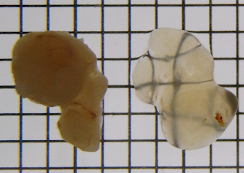
\includegraphics[width=0.7\linewidth]{fig/chapter1/lucid}
	\caption{Transparent specimen}
	\label{fig:lucid}
\end{figure}

\begin{figure}[H]
	\centering
	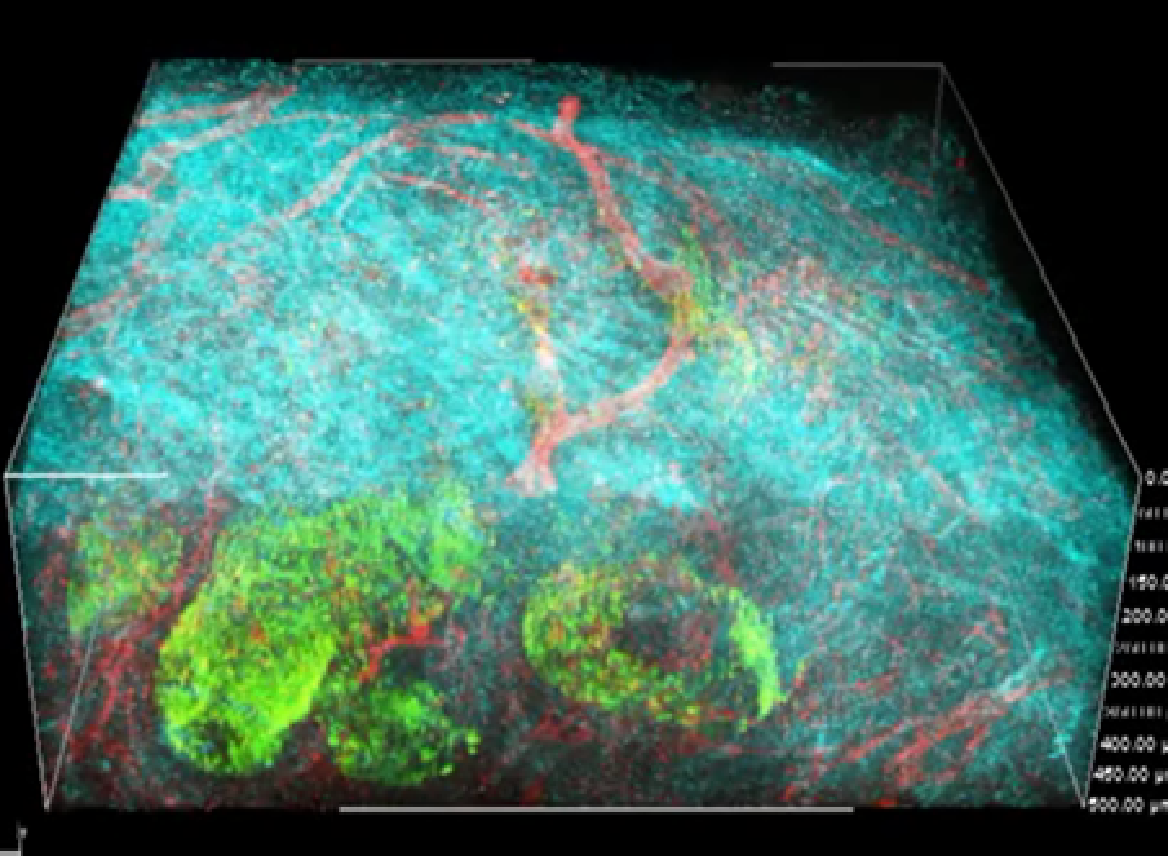
\includegraphics[width=0.7\linewidth]{fig/chapter1/microscope}
	\caption{Image taken by multi focus microscope}
	\label{fig:microscope}
\end{figure}


\section{本研究の目的}
本研究の目的は,内視鏡生検を透明にして深層学習を利用して癌を見落とさない診断方法を開発することである.組織透明化技術LUCIDを用いて検体を丸ごと透明化し,共焦点顕微鏡で観察することで検体の内部まで3次元情報として解析することができる.

\begin{figure}[H]
	\centering
	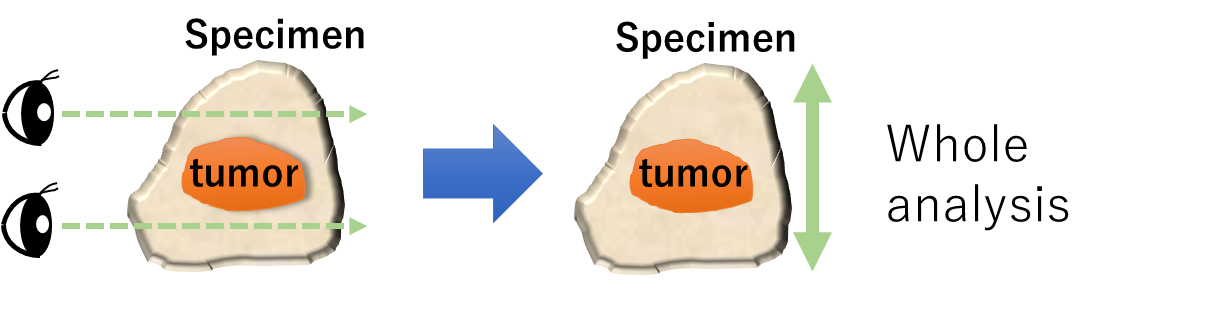
\includegraphics[width=0.7\linewidth]{fig/chapter1/whole_image_analysis}
	\caption{Schematic of whole image analysis}
	\label{fig:wholeimageanalysis}
\end{figure}

透明化されたサンプルを共焦点顕微鏡で撮影すると,従来のカットする手法に換算して1000カットに相当する.そのため,得られる顕微鏡撮影像が従来の2,3カットに対して数100倍となるので,専門医が診断をするには負担が大きくなってしまう.そこで,人工知能(Artificial Intelligence: AI)が3次元画像を解析して病変を検知し,専門医に提示することで病変の見落としリスクがゼロになる診断支援システムを開発することが本研究の目的である.


生検ではないAIを用いた内視鏡の診断支援では,内視鏡カメラの画像解析を行う事例がある.国立がん研究センターとNECが共同で開発したシステムがある\cite{要出典}.しかし診断を確定するには生検が必須であり,生検の病理診断にマンパワーが必要になっている.
生検のAIによる診断アルゴリズム開発の先行研究としては,胃がん,肺がんや乳がん,骨髄などの生検をディープラーニングで境界認識するものががあり,90\%程度の正解率を出している\cite{要出典}.これは専門医と同程度の精度がすでに達成しているが,データセットとして提供されているのは単純の形状のものが多い.

本研究では生検の3次元画像を解析することで2次元画像では判断の難しいものを3次元特有の情報を用いることで判定精度を上げることを目標とする.

機械学習を行うためには教師データを用意する必要があるが,医療データはアノテーションされていないことが多い.3次元画像を解析する先行研究としては,CTやMRI画像が上げられる.CTやMRIの場合は画像の分解能が顕微鏡像よりも低く,深さ方向にも30程度である.本研究は透明化処理した生検を蛍光顕微鏡で撮影するため分解能が高く,深さ方向にも400~700枚が撮影することができる.このためディープラーニングで解析するときに計算のメモリに乗らないという問題が生じるため解析手法を工夫して計算量がなるべく減るようにしなければいけない.今回は時系列処理で使われる手法と画像処理の手法を組み合わせて用いることで,大きな画像サイズでも解析することができるようにした.


深層学習で解析を行う場合はデータを大量に準備する必要がある.今回のように,新しい撮影手法であったり,希少な病気であったりすると医療データを数多く集められないことがある.さらに画像データだけでなく,その画像に教師ラベルを貼る(アノテーション)必要がある.画像と,その教師ラベルのセットを数万枚と集めることができたら高い精度が出るという報告が多くあるが,少ない教師データで識別精度を上げることは深層学習において困難とされている.教師データの作成が困難であるだけでなく,少量データである場合は,その教師データが医師によってばらつきがある場合は,教師データを作成した医師の判断が大きく反映されてしまい,必ずしも真であると断言することができなくなってしまう.これらの課題があるため医療画像における深層学習を用いた診断システムは,大量にデータを用意するまでの時間や人的コストを大きく払うことになっているのが現状である.

本研究でこの課題に取り組んだ.教師ラベルを必要とせず,画像の構造的な特徴のパターンを学ぶ,教師なし学習の手法と,これまでの教師ラベルを使った学習とを組み合わせた,半(弱)教師あり学習を行った.構造的なパターンは3次元画像であることを活用し,教師なし学習については,病理画像が正常から異常になる過程には連続的な性質があることを活用して正常と異常の分布が作れるようにした.


最後にこの深層学習による腫瘍の検出結果を医師が診断する際のサポートになるように可視化する.深層学習は,よく判断の理由が分からないためブラックボックスと呼ばれ,信頼性が求められる場面では利用に対して不安視されることがある.そのため腫瘍と正常の診断の判断の理由が可視化して,どの部分に注目しているかを医師に見せる.医師の負担を減らすためのスクリーニングとして利用するために,明らかに正常のものと,腫瘍かもしれない領域とを区別して,腫瘍かもしれない部分を医師に提示する.3次元画像であるから医師が診断するには,全ての断面を確認することは現実的に不可能である.腫瘍を見落とさないように,深層学習によって,腫瘍がある確率の高い断面を提示して診断支援を行う.

本研究の目的は内視鏡生検を透明にして深層学習を利用して癌を見落とさない診断方法を開発することである.組織透明化技術LUCIDを用いて検体を丸ごと透明化し,レーザー顕微鏡で観察することで,顕微鏡の解像度で検体の内部まで3次元情報として解析することができる.

透明化されたサンプルをレーザー顕微鏡で撮影すると,従来のカットする手法に換算して1000カットに相当するため,得られる顕微鏡撮影像が従来の2,3カットに対して数百倍となるので,専門医が診断をするには負担が大きくなってしまう.したがって,AI(人工知能)が3次元画像を解析して病変を検知し専門医に提示することで病変の見落としリスク(偽陰性)がゼロになる診断支援システムを開発することが本研究の目的である.

深層学習で解析を行う場合はデータを大量に準備する必要がある.今回のように,新しい撮影手法であったり,希少な病気であったりすると医療データを数多く集められないことがある.さらに画像データだけでなく,その画像に教師ラベルを貼る(アノテーション)必要がある.画像と,その教師ラベルのセットを数万枚と集めることができたら高い精度が出るという報告が多くあるが,少ない教師データで識別精度を上げることは深層学習において困難とされている.教師データの作成が困難であるだけでなく,少量データである場合は,その教師データが医師によってばらつきがある場合は,教師データを作成した医師の判断が大きく反映されてしまい,必ずしも真であると断言することができなくなってしまう.これらの課題があるため医療画像における深層学習を用いた診断システムは,大量にデータを用意するまでの時間や人的コストを大きく払うことになっているのが現状である.

本研究でこの課題に取り組んだ.教師ラベルを必要とせず,画像の構造的な特徴のパターンを学ぶ,教師なし学習の手法と,これまでの教師ラベルを使った学習とを組み合わせた,半(弱)教師あり学習を行った.構造的なパターンは3次元画像であることを活用し,教師なし学習については,病理画像が正常から異常になる過程には連続的な性質があることを活用して正常と異常の分布が作れるようにした.
